Como visto no capítulo anterior [\ref{chapter:ruby_e_suas_bibliotecas}] a maior parte das bibliotecas do 
\emph{Ruby} são distribuídas na forma de \emph{gemas} (\emph{gems}) e também vimos na seção 
[\ref{subsection:gem}] deste mesmo cápitulo que o \emph{gem} é um sistema de distribuição sinilar ao 
\emph{\href{https://packages.qa.debian.org/a/apt.html}{apt-get}} que facilita o compartilhamento e a 
instalação das \emph{gemas}. 

Deste modo, como já temos alguns conhecimento básicos sobre bibliotecas e sobre o \emph{Ruby}, neste cápitulo 
iremos apresentar um tutorial básco de como se pode criar uma \emph{gema} do \emph{Ruby}.

A ideia de se criar uma gema geralmente vai surgir quando se perceber que uma determinadade funcionalidade de
um sistema também é utilizado em vários outros sistemas que a equipe trabalha. Por este motivo visando a economia
de tempo se faz a criação de bibliotecas para que não seja mais necessário copiar e colar códigos 
% (\emph{Ctrl + C}, \emph{Ctrl + V}).

Para se criar uma gema (biblioteca do \emph{Ruby}) precisamos inicialmente entender para que serve cada um
de seus compoentes e isso será explicado logo a seguir na seção 
‘‘\ref{section:estrutura_de_uma_gema} Estrutura de uma gema'', e depois em seguida veremos um modelo de criação 
na seção ‘‘\ref{section:modelo_de_criação} Modelo de Criação''.

\section{Estrutura de uma gema}
\label{section:estrutura_de_uma_gema}

Uma gema do \emph{Ruby} obrigatoriamente deve possui um nome, um número de versão e uma plataforma.
Internamente ela possui código, documentação e o \emph{\textbf{gemspec}}, onde a sua estrutura geralmente é 
organizada em 3 arquivos bases: o \emph{\textbf{gemspec}}, o \emph{\textbf{Rakefile}} e o 
\emph{\textbf{README}}, e em 3 diretórios principais: \emph{\textbf{bin}}, \emph{\textbf{lib}}, e 
\emph{\textbf{test}} ou \emph{\textbf{spec}}. Na listagem abaixo veremos para que serve cada um destes
arquivos e diretórios.

\begin{itemize}

 \item O \emph{\textbf{gemspec}} é um arquivo do tipo ‘‘\emph{.gemspec}'' que possui as informações básicas 
 de uma gema, como por exemplo o seu nome, sua descrição, seu autor, seu endereço, e suas dependências.

 \item O \emph{\textbf{bin}} é um diretório que possui os arquivos executáveis da gema que serão 
 carregados quando a gema for instalada.

 \item O \emph{\textbf{lib}} é um diretório que possui todos os códigos \emph{Ruby} referente ao 
 funcionamento da gema.

 \item O \emph{\textbf{test}} ou \emph{\textbf{spec}} é um diretório que possui todos os códigos \emph{Ruby} 
 de testes, onde eles podem ser executados manualmente ou por meio do \emph{Rakefile}.

 \item O \emph{\textbf{Rakefile}} é um arquivo que possui código \emph{Ruby} que faz a otimização de algumas
 funcinalidades por meio da execução do programa \emph{\href{https://github.com/jimweirich/rake}{rake}} 
\footnote{rake: \url{https://github.com/jimweirich/rake}}. Um exemplo é a execução de todos os arquivos 
de testes do diretório \emph{test} ou \emph{spec}.

 \item O \emph{\textbf{README}} é um arquivo que usualmente possui a documentação da gema que está dentro do 
 código. Geralmente ele é gerado automaticamente quando a gema é instalada. A maioria das gemas possuem
 a documentação \emph{\href{http://rdoc.sourceforge.net/doc/}{RDoc}} 
 \footnote{RDoc: \url{http://rdoc.sourceforge.net/doc/}}, e as outras em menoria possuem a documentação 
 \emph{\href{http://yardoc.org/}{YARD}} \footnote{YARD: \url{http://yardoc.org/}} 
 [\citeonline{guide_what_is_a_gem_rubygems}].

\end{itemize}

\section{Modelo de criação}
\label{section:modelo_de_criação}

O primeiro passo para se criar uma gema é construir uma solução de um certo problema que geralmente vai
ser utilizado. Por exemplo a função que calcula a raiz quadrada de um número é uma funcionalidade que 
usualmente utilizamos quando estamos fazendo cálculos. 

Após encontrar uma ideia para a criação de uma gema deve-se elaborar um projeto, fazendo o levantamento 
de requisitos, o \emph{design}, a implementação, os testes e a entrega.

Por simplificação nesta sub-seção somente apresentaremos a parte de implementação do modelo de criação de uma
gema, mas nunca se deve esquecer de seguir todos os passos de um projeto, desde o momento da formação da 
ideia até a sua entrega, pois caso esses passos não sejam seguidos, os riscos de se 
perder recursos, como tempo e dinheiro, é muito alto.

Para facilitar a apresentção deste modelo utilizaremos como exemplo a gema 
\emph{\href{https://github.com/toshikomura/gemtranslatetoenglish/tree/without_path}{gemtranslatetoenglish}} 
\footnote{gemtranslatetoenglish : \url{https://github.com/toshikomura/gemtranslatetoenglish/tree/without_path}} que tem 
como objetivo fazer a tradução de um texto em português para um texto em inglês. 

Futuramente pretendemos aumentar o vocabulário da gema de exemplo, mas até o momento de término deste 
trabalho, ela possuía somente a tradução de duas palavras, ‘‘\emph{OI}'' para ‘‘\emph{HELLO}'' e 
‘‘\emph{MUNDO}'' para ‘‘\emph{WORLD}''. Apesar de possuir pouco vocabulário, a gema ‘‘\emph{gemtranslatetoenglish}''
será suficiente para a aparesentação do tutorial deste trabalho. 

Nesta sub-seção apresentaremos primeiramente como se pode criar uma estrtura básica de uma gema na sub-seção 
‘‘\ref{subsection:criando_a_estrutura} Criando a Estrutura'', em seguida mostraremos na 
‘‘\ref{subsection:gemspec} Gemspec'' como se deve editar o arquivo \emph{.gemspec}, depois iremos apresentar 
como se pode desenvolver o código de funcionalidades de uma gema na sub-seção ‘‘\ref{subsection:lib} Lib'', 
sequêncialmente apresentaremos na sub-seção ‘‘\ref{subsection:test_ou_spec_e_arquivo_rakefile} Teste ou Spec e 
Arquivo Rakefile'' como implementar o código de testes, em seguida na sub-seção 
‘‘\ref{subsection:execução_de_testes} Execução de Testes'' apresentaremos uma forma para executar os testes, 
depois apresentaremos uma forma de testar a gema através da ferramenta \emph{IRB} na sub-seção 
‘‘\ref{subsection:irb} IRB'', e por fim na sub-seção ‘‘\ref{subsection:exemplo_de_uso_de_gemtranslatetoenglish} 
Exemplo de Uso de gemtranslatetoenglish'' apresentaremos um exemplo de uso da gema 
‘‘\emph{gemtranslatetoenglish}'' dentro de um projeto.

\subsection{Criando a Estrutura}
\label{subsection:criando_a_estrutura}

O primeiro passo é fazer a criação da estrutura da gema e isso pode ser feito de forma manual ou automática. 
A forma manual implica em criar todos os diretórios e arquivos manualmente e a forma automática implica na
execução de um simples comando. Contudo podemos perceber qua a forma manual não é muito aconselhável e 
por esse motivo utilizaremos a forma automática que pode ser feita no terminal com a execução do comando
que pode ser vista no código ‘‘Código \ref{lst:cria_gema_forma_geral} - Cria Gema Forma Geral''.

\lstinputlisting[ style=customBash, caption={Cria Gema Forma Geral}, label={lst:cria_gema_forma_geral}]
{codigos/cria_gema_forma_geral.sh}

No caso da nossa gema de exemplo foi feita a execução do seguinte comando apresentado no código 
‘‘Código \ref{lst:cria_gema_gemtranslatetoenglish} - Cria Gema gemtranslatetoenglish''.

\lstinputlisting[ style=customBash, caption={Cria Gema gemtranslatetoenglish}, label={lst:cria_gema_gemtranslatetoenglish}]
{codigos/cria_gema_gemtranslatetoenglish.sh}

Ao se fazer a execução do comando ‘‘\emph{bundle gem gemtranslatetoenglish}'' obtemos a seguinte estrutura de gema mostrada 
no código ‘‘Código \ref{lst:execucao_que_cria_gema_gemtranslatetoenglish} - Execução que cria gema gemtranslatetoenglish''.
% na imagem ‘‘Figura \ref{fig:execucao_que_cria_gema_gemtranslatetoenglish} - Execução que cria gema gemtranslatetoenglish''.

\lstinputlisting[ style=customBash, caption={Execução que cria gema gemtranslatetoenglish}, label={lst:execucao_que_cria_gema_gemtranslatetoenglish}]
{codigos/execucao_que_cria_gema_gemtranslatetoenglish.sh}

\begin{comment}
\begin{figure}[ht]
  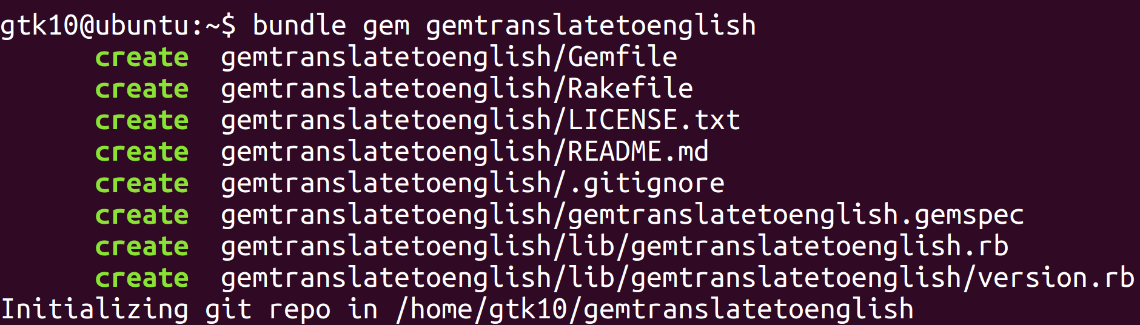
\includegraphics[scale=0.4]{images/execucao_que_cria_gema_gemtranslatetoenglish}
  \caption{Execução que cria gema gemtranslatetoenglish}
  \label{fig:execucao_que_cria_gema_gemtranslatetoenglish}
\end{figure}
\end{comment}

\subsection{Gemspec}
\label{subsection:gemspec}

Agora que possuimos a estrutura da gema, devemos fazer a edição do arquivo \emph{\textbf{gemspec}} 
para informar os dados básicos da gema e isso pode ser feito editando o arquivo ‘‘ 'nome da gema'.gemspec ''. 
No nosso exemplo fizemos a edição do arquivo ‘‘gemtranslatetoenglish.gemspec'' resultado no arquivo mostrado 
no código ‘‘Código \ref{lst:gemspec_gemtranslatetoenglish} - gemspec gemtranslatetoenglish''
%na imagem ‘‘Figura \ref{fig:gemspec_gemtranslatetoenglish} - gemspec gemtranslatetoenglish''
, onde cada linha será explicada com mais detalhes logo a seguir.

\lstinputlisting[ style=customBash, caption={gemspec gemtranslatetoenglish}, label={lst:gemspec_gemtranslatetoenglish}]
{codigos/gemtranslatetoenglish/gemtranslatetoenglish.gemspec}

\begin{comment}
\begin{figure}[ht]
  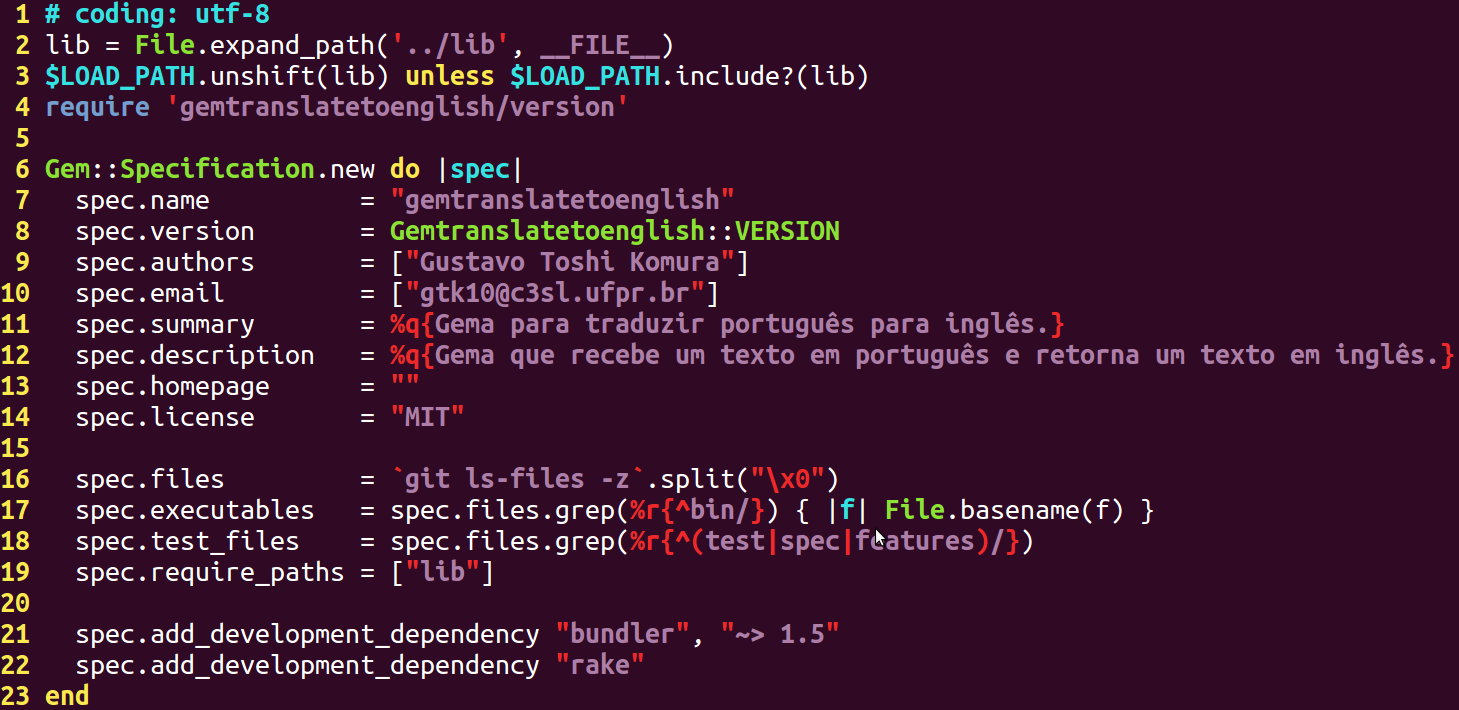
\includegraphics[scale=0.3]{images/gemspec_gemtranslatetoenglish}
  \caption{gemspec gemtranslatetoenglish}
  \label{fig:gemspec_gemtranslatetoenglish}
\end{figure}
\end{comment}

\begin{itemize}

 \item ‘‘\emph{\# coding: utf-8}'' na linha ‘‘1'' indica que o texto do arquivo está no formato \emph{UTF-8}.
 
 \item ‘‘\emph{lib = File.expand\_path('..\/lib', \_\_FILE\_\_)}'' na linha ‘‘2'' indica onde se encontra o 
 diretório \emph{\textbf{lib}} da gema.
 
 \item ‘‘\emph{\$LOAD\_PATH.unshift(lib) unless \$LOAD\_PATH.include?(lib)}'' na linha ‘‘3'' faz o 
 carregamento dos arquivos que estão no diretório \emph{\textbf{lib}} caso o diretório já esteja definido.
 
 \item ‘‘ \emph{require 'gemtranslatetoenglish/version'} '' na linha ‘‘4'' requisita o arquivo de versão da
 gema.
 
 \item ‘‘\emph{Gem::Specification.new do |spec|} ... end'' da linha ‘‘6'' a ‘‘23'' define a especifação da
 gema como \emph{spec}, ou seja, ao invés de escrever ‘‘\emph{Gem::Specification}'' a todo momento que for 
 definir uma especificação da gema se escreve somente ‘‘\emph{spec}''.
 
 \item ‘‘\emph{spec. }'' da linha ‘‘7'' a linha ‘‘14'' defini-se espcificações básicas da gema, como nome,
 versão, autor, e-mail do autor, breve descrição, descrição completa, página e tipo de licença.
 
 \item ‘‘\emph{spec.files = `git ls-files -z`.split("$\backslash$x0")}'' na linha ‘‘16'' indica os arquivos
 que devem ser incluídos na gema. Esses arquivos são incluídos dinâmicamente através do comando 
 ‘‘\emph{git ls-files -z}'' que traz como resultado todos os arquivos que estão naquele repositório 
 colocando entre as \emph{PATH}s deles o caracter ‘‘\emph{$\backslash$0}'' 
 (\emph{line termination on output}). Por consequência com a adição do comando \emph{Ruby} 
 ‘‘\emph{.split("$\backslash$x0")}'', que indica a divisão por ‘‘\emph{$\backslash$0}'', os arquivos 
 adicionados na gema são todos que estão no repositório. 
 
 Para se adicionar arquivos no repositório é necessário executar o comando ‘‘\emph{git add PATH}'', 
 onde \emph{PATH} é o caminho do arquivo que se deseja adicionar no repositório.
 
 \item ‘‘\emph{spec.executables = ...}'' e ‘‘\emph{spec.tes\_files = ...}'' nas linhas ‘‘17'' e ‘‘18'' 
 indicam os arquivos executáveis e os arquivos de teste respectivamente, e também indica que ambos devem
 ter permissão de execução, pois caso este arquivos não possuam essa permissão, eles não são incluídos 
 na gema.
 
 \item ‘‘\emph{spec.require\_paths = ["lib"]}'' requisita o diretório da \emph{\textbf{lib}} da gema.
 
 \item ‘‘\emph{spec.add\_development\_dependency = ...}'' nas linhas ‘‘21'', ‘‘22'' e ‘‘23'' requistam como 
 dependências as gemas ‘‘\emph{bundle}'' versão ‘‘1.5'', ‘‘\emph{rake}'' e ‘‘\emph{action\_controller}''
 respectivamente.
 
\end{itemize}

\subsection{Desenvolvimento de código de funcionalidade ou teste}
\label{subsection:desenvolvimento_de_codigo_de_funcionalidade_ou_teste}

Nesse momento podemos tomar 2 caminhos e isso depende da metodologia de projeto que adotadomos no inicio 
do desenvolvimento, ou seja, é nesse momento que podemos desenvolver o código das funcinalidades
ou implementar o código de testes. 

Na metodologia tradicional se faz a implementação do código de funcionalidades e depois se
desenvolve o código para testar essas funcionalidades. Por outro lado na metodologia voltada para 
testes, se implementa o código de testes para depois se desenvolver o código de funcionalidades.

Seguindo a metodologia tradicional, primeiramente iremos fazer o código das funcinalidades da gema.
Depois ao terminar de criar essas funcionalidades iremos elaborar os arquivos testes, mas nada o impede
de desenvolver os códigos de testes que serão apresentado na sub-sub-seção 
‘‘\ref{subsection:test_ou_spec_e_arquivo_rakefile} Test ou Spec e arquivo Rakefile'' antes de 
desenvolver os códigos de funcionalidade mostrados na sub-sub-seção ‘‘\ref{subsection:lib} Lib''.

\subsection{Lib}
\label{subsection:lib}

Nesta sub-seção vamos aprender a fazer o código de funcionalidade de uma gema, mas caso deseje fazer 
primeiro os códigos de casos de testes, pode-se consultar a sub-seção 
‘‘\ref{subsection:test_ou_spec_e_arquivo_rakefile} Test ou Spec e arquivo Rakefile'' e depois retornar
para esta sub-seção para dar continuidade ao desenvolvimento.

Caso esse código seja por meio de código \emph{Ruby} devemos fazer a edição e criação de arquivos no 
diretório \emph{\textbf{lib}}. Este diretório obrigatoriamente deve possuir um arquivo 
‘‘ 'nome da gema'.rb '' e um diretório também com o nome da gema. Dentro do diretório devemos criar um 
arquivo de versão. No nosso exemplo isso pode ser verificado consultando no código ‘‘Código 
\ref{lst:execucao_que_cria_gema_gemtranslatetoenglish} - Execução que cria gema gemtranslatetoenglish'' 
que após a execução do comando ‘‘\emph{bundle gem gemtranslatetoenglish}'' é feita a criação do arquivo 
‘‘\emph{lib/gemtranslatetoenglish.rb}'' na linha ‘‘8'', e o drietório ‘‘\emph{lib/gemtranslatetoenglish}'' 
com o arquivo ‘‘\emph{version}'' dentro dele na linha ‘‘9''.

O arquivo ‘‘\emph{version}'' somente define a versão que a gema está, onde no nosso exemplo da gema 
‘‘\emph{gemtranslatetoenglish}'' a primeira versão é a ‘‘\emph{0.0.1}''. 

Basicamente a descrição da versão de uma gema é uma string com números e pontos. Também é permitido 
colocar ao final a palavra chave ‘‘\emph{pre}'' caso seja um pré-lançamento de alguma versão, como 
por exemplo ‘‘\emph{1.0.0.pre}'' é um pré-lançamento da versão ‘‘\emph{1.0.0}''.

O \emph{Rubygems} recomenda seguir as seguintes politicas mencionadas logo abaixo que foram consultadas
em \emph{\href{http://guides.rubygems.org/patterns/\#semantic-versioning}{semantic-versioning}}
\footnote{semantic-version: \url{http://guides.rubygems.org/patterns/\#semantic-versioning}} e em
\emph{\href{http://guides.rubygems.org/specification-reference/\#version}{specification-reference-version}}
\footnote{specification-reference-version: \url{http://guides.rubygems.org/specification-reference/\#version}}.

\begin{itemize}
 \item PATH : “0.0.X” para pequenas alterações, como por exemplo correção de pequenos \emph{bugs}.
 \item MINOR: “0.X.0” para médias alterações, como por exemplo alteração/adição de funcionalidades.
 \item MAJOR: “X.0.0” para grandes alterações, como por exemplo remoção de alguma funcionalidade.
\end{itemize}

Antes de continuarmos a codificação das funcionalidades da gema precisamos entender algumas diferenças
básicas de conceitos do \emph{Ruby}, como por exemplo a diferença entre \emph{module} e \emph{class},

Os ‘‘\emph{modules}'' ou módulos se preferir, definem um conjunto de métodos e constantes. Podemos 
dizer que os métodos dos módulos são estáticos, pois não precisamos instanciar o módulo para usar os
seus métodos. Contudo podemos dizer que os módulos são parecidos com o conceito de interface do 
\emph{Java}. 

Por outro lado a ‘‘\emph{class}'' também é um conjunto de métodos e constantes, no 
entanto para usar os seus métodos e constantes é necessário instância-lá, ou seja, é necessário criar 
um objeto da ‘‘\emph{class}'' na memória para usar os seus respectivos métodos. 

Contudo por essas características podemos dizer que uma ‘‘\emph{class}'' é basicamente 
uma subclasse do ‘‘\emph{module}'', pois a ‘‘\emph{class}'' possui 4 métodos a mais, que no caso são 
os métodos ‘‘\emph{initialize()}'', ‘‘\emph{superclass()}'', ‘‘\emph{allocate()}'' e ‘‘\emph{to\_yank()}''.

Agora que temos alguns conceitos do \emph{Ruby} apresentados, podemos continuar com a implementação 
da nossa gema. 

No arquivo ‘‘ lib/'nome da gema'.rb '' temos a possibilidade de escerver todas as 
funcinalidades desejadas. No nosso exemplo o arquivo ‘‘lib/gemtranslatetoenglish.rb'' é mostrado no código 
‘‘Código \ref{lst:gemtranslatetoenglish.rb} - gemtranslatetoenglish.rb'', onde cada linha é explicado 
logo a seguir.

\lstinputlisting[ style=customRuby, caption={gemtranslatetoenglish.rb}, label={lst:gemtranslatetoenglish.rb}]
{codigos/gemtranslatetoenglish/lib/gemtranslatetoenglish.rb}

\begin{itemize}

 \item ‘‘\emph{require "gemtranslatetoenglish/version"} '' na linha ‘‘1'' é feita a requsição do arquivo de
 versão.
 
 \item ‘‘\emph{require "gemtranslatetoenglish/translatetoenglish.rb"} '' na linha ‘‘4'' é feita a requisição
 do arquivo ‘‘\emph{translatetoenglish.rb}'' contido no diretório ‘‘gemtranslatetoenglish''.
 
 \item ‘‘\emph{module Gemtranslatetoenglish ... end}'' na linha ‘‘6'' a ‘‘8'' define o módula da gema.
 
 \item ‘‘\emph{ActionController::Base.helper Gemtranslatetoenglish::Helpers::Translatetoenglish}'' na linha 
 ‘‘10'' define uma extensão da classe ‘‘ActionController::Base.helper'', onde a classe a ser acrescentada é
 a classe ‘‘\emph{Gemtranslatetoenglish::Helpers::Translatetoenglish}''. Esta extensão foi adicionada
 para que no momento de uso das funcionalidades da gema na \emph{view} não fosse necessário fazer a chamada 
 de tradução  escrevendo toda \emph{PATH}. Por exemplo para chamar a função de tradução, ao invés
 de chamar ‘‘\emph{gemtranslatetoenglish.Translatetoenglish.translate(‘Oi’)}'', se faz a chamada 
 ‘‘\emph{translate(‘Oi’)}'' na \emph{view}.
 
\end{itemize}

Podemos perceber que o comando ‘‘\emph{require}'' é utilizado para fazer a chamada de código de outros 
arquivos e isso serve para fazer a modularização da gema que no caso é uma boa prática de programação.

Podemos supor que desenvolvemos uma gema e depois de um certo tempo precisamos fazer a manutenção do 
seu código. Neste caso se não modularizamos a gema, a correção de \emph{bugs} ou mesmo a adição de 
novas funcionalidades torna-se uma tarefa muito complexa, pois não existe nenhuma organização 
estrutural na gema preparada para facilitar esse tipo de operação. 

Observando novamente o código ‘‘Código \ref{lst:gemtranslatetoenglish.rb} - gemtranslatetoenglish.rb'' 
podemos perceber que na linha ‘‘4'' foi feito o \emph{require} do arquivo 
‘‘\emph{gemtranslatetoenglish/translatetoenglish.rb}'' que será mostrado no código ‘‘Código 
\ref{lst:translatetoenglish.rb} - translatetoenglish.rb'' e explicado logo a seguir.

\lstinputlisting[ style=customRuby, caption={translatetoenglish.rb}, label={lst:translatetoenglish.rb}]
{codigos/gemtranslatetoenglish/lib/gemtranslatetoenglish/translatetoenglish.rb}

\begin{itemize}

  \item ‘‘\emph{module ... end} nas linhas ‘‘1'', ‘‘2'' e ‘‘3'' até as linhas ‘‘44'', ‘‘45'' e ‘‘46'' 
  define a árvore de módulos ‘‘\emph{Gemtranslatetoenglish}'' na raiz, ‘‘\emph{Helpers}'' no segundo 
  nível e depois ‘‘\emph{Translatetoenglish}'' no terceiro nível.
  \item ‘‘\emph{def translate( phrase) ... end}'' da linha ‘‘5'' até a linha ‘‘42'' define a função de 
  tradução da gema, onde foi definido somente duas traduções, ‘‘\emph{OI}'' para ‘‘\emph{HELLO}'' 
  e ‘‘MUNDO'' para ‘‘\emph{WORLD}''.
  
  A árvore definida no código ‘‘Código \ref{lst:translatetoenglish.rb} - translatetoenglish.rb'' foi 
  necessário por causa do código inserido na linha ‘‘10'' 
  ‘‘\emph{ActionController::Base.helper Gemtranslatetoenglish::Helpers::Translatetoenglish}''
  no código ‘‘Código \ref{lst:gemtranslatetoenglish.rb} - gemtranslatetoenglish.rb'' que serve para 
  evitar a necesseidade de escrever a \emph{PATH} completa na \emph{view} para chamar uma função 
  da gema na \emph{view}.
  
\end{itemize}

\subsection{Test ou Spec e arquivo Rakefile}
\label{subsection:test_ou_spec_e_arquivo_rakefile}

Lembrando que podemos fazer o desenvolvimento de código de funcinalidades ou o código de testes, e isso é
dependente da metodologia adotada no inicio do projeto, caso queira fazer o código de funcionalidade antes
do desenvolvimento dos casos de teste se pode consutar a sub-seção ‘‘\ref{subsection:lib} Lib''.

Para se fazer os testes, deve-se criar os arquivos de testes dentro do diretório ‘‘\emph{test}'' ou se 
preferir ‘‘\emph{spec}''. Não existe um padrão especificado, mais recomenda-se criar um arquivo de 
teste com o nome ‘‘\emph{test/test\_‘definição do teste'.rb}''. No nosso exemplo criamos o arquivo 
‘‘\emph{test/test\_check\_translate.rb}'' que podemo ver no código ‘‘\ref{lst:test_check_translate.rb} - 
Testa translate gemtranslatetoenglish'' explicado logo a seguir.

\lstinputlisting[ style=customRuby, caption={Testa translate gemtranslatetoenglish}, label={lst:test_check_translate.rb}]
{codigos/gemtranslatetoenglish/test/test_check_translate.rb}

\begin{itemize}

 \item Nas linhas ‘‘1'', ‘‘2'' e ‘‘3'' nos códigos ‘‘ \emph{require ‘...'} '' requisitamos respectivamente o 
 ‘‘\emph{autorun}'' da gema ‘‘\emph{minitest}'' que utilizaremos para realizar os testes, 
 ‘‘\emph{action\_controller}'' que utilizamos para evitar a obrigação de digitar a ‘‘\emph{PATH}'' completa 
 na \emph{view}, e ‘‘\emph{gemtranslatetoenglish}'' que é a nossa gema de exemplo.
 
 \item Na linha ‘‘5'' fomos obrigados a fazer o ‘‘\emph{include}'' do módulo 
 ‘‘\emph{Gemtranslatetoenglish::Helpers::Translatetoenglish}'' para que todas as funções do módulo fossem 
 disponiblizadas para uso e no nosso caso era o método ‘‘\emph{translate()}''.
 
 \item Da linha ‘‘7'' a linha ‘‘16'' é definido a classe de teste \emph{TranslateTest} que herda as 
 características de ‘‘\emph{MiniTest::Unit::TestCase}''.
 
 \item Da linha ‘‘8'' a linha ‘‘11'' é definido o teste por palavra, onde é verificado através do 
 ‘‘\emph{assert\_equal}'' se a ‘‘\emph{string}'' esperada no primeiro parâmetro é retornadda pela chamada 
 da função ‘‘\emph{Gemtranslatetoenglish::Helpers::Translatetoenglish.translate()}'' no segundo parâmetro.
  
 \item Da linha ‘‘12'' a linha ‘‘15'' é definido o teste por texto, onde é verificado através do 
 ‘‘\emph{assert\_equal}'' se a ‘‘\emph{string}'' esperada no primeiro parâmetro é retornadda pela chamada 
 da função ‘‘\emph{Gemtranslatetoenglish::Helpers::Translatetoenglish.translate()}'' no segundo parâmetro.
 
\end{itemize}

Agora que temos o nosso arquivo de teste, precisamos criar o arquivo ‘‘\emph{Rakefile}'' e executar o 
comando ‘‘\emph{rake}'' para realizarmos os testes.

No nosso exemplo da gema ‘‘\emph{gemtranslatetoenglish}'' desenvolvemos o seguinte arquivo 
‘‘\emph{Rakefile}'' que pode ser visualizado no código ‘‘Código \ref{lst:rakefile} - 
Rakefile gemtranslatetoenglish'' sendo explicado os detalhes logo a seguir.

\lstinputlisting[ style=customRuby, caption={Rakefile gemtranslatetoenglish}, label={lst:rakefile}]
{codigos/gemtranslatetoenglish/Rakefile}

\begin{itemize}

\item Nas linhas ‘‘1'' e ‘‘2'' nos códigos ‘‘ \emph{require ‘...'} '' requisitamos respectivamente o 
 ‘‘\emph{gem\_tasks}'' do ‘‘\emph{bundler}'' e ‘‘\emph{testtask}'' do ‘‘\emph{rake}'', ambos necessários para
 a execução dos testes.
 
 \item Da linha ‘‘4'' a ‘‘6'' é feito a criação de uma nova ‘‘\emph{task}'' de teste para cada arquivo 
 que esteja no diretório ‘‘\emph{test}''.
 
 \item A linha ‘‘5'' com o código ‘‘ \emph{t.libs << ‘test'} '' inidica que os arquivos de testes estão no 
 diretório ‘‘\emph{test}''.

 \item Por fim na linha ‘‘9'' com o código ‘‘\emph{task :default => :test}'' se requisita a execução 
 dos testes.
 
\end{itemize}

\subsection{Execução de testes}
\label{subsection:execução_de_testes}

Antes de realizarmos os testes, precisamos criar a gema com comando ‘‘\emph{gem build 'nome da gema'.gemspec}'' 
e fazer a instalação com o comando ‘‘\emph{sudo gem install 'nome da gema'-'versão da gema'.gem}''. No nosso 
caso é fazer a crição e a instalação da gema ‘‘\emph{gemtranslatetoenglish}'', que pode ser feito da mesma 
forma como apresentado no código ‘‘Código \ref{lst:execucao_que_cria_e_instala_gemtranslatetoenglish} - Execução 
gem install gemtranslatetoenglish''.

\lstinputlisting[ style=customBash, caption={Execução que Cria e Instala gemtranslatetoenglish}, label={lst:execucao_que_cria_e_instala_gemtranslatetoenglish}]
{codigos/execucao_que_cria_e_instala_gemtranslatetoenglish.sh }

Agora após ter implementado o código das funcionalidades, o arquivo de teste 
‘‘\emph{test/test\_check\_translate.rb}'', o arquivo \emph{Rakefile}, e ter feito a criação e a instalação 
da gema de exemplo, podemos realizar os testes com a execução do comando ‘‘\emph{rake}'' no terminal. 

Com a execução dos testes obtemos como resultado o código ‘‘Código 
\ref{lst:execucao_rake_gema_gemtranslatetoenglish} - Execução rake gema gemtranslatetoenglish'' explicado 
logo a seguir.

\lstinputlisting[ style=customBash, caption={Execução rake gema gemtranslatetoenglish}, label={lst:execucao_rake_gema_gemtranslatetoenglish}]
{codigos/execucao_rake_gema_gemtranslatetoenglish.sh }

\begin{itemize}

 \item Na linha ‘‘1'' é feito a execução do comando ‘‘\emph{rake}'' para se realizar os testes.
 
 \item Na linha ‘‘9'' é mostrado que foram feitos 2 testes, no caso os 2 que definimos no código 
 ‘‘\ref{lst:test_check_translate.rb} - Testa translate gemtranslatetoenglish'' nas linhas 
 ‘‘8'' a ‘‘11'' no teste ‘‘\emph{test\_world\_translation}'' e nas linhas ‘‘12'' a ‘‘15'' no teste 
 ‘‘\emph{test\_text\_translation}''. Também é apresentado na linha ‘‘9'' que foram feitos 4 
 ‘‘\emph{assertions}'', no caso dois para cada caso de teste feitos por meio do ‘‘\emph{assert\_equal}''.
 E além disso é apresentado que não ocorreram  \emph{failures}''), ‘‘\emph{errors}'' e ‘‘\emph{skips}''.
 
\end{itemize}

Deste modo ao se realizar estes testes garantimos que pelo menos a função ‘‘\emph{translate()}'' da gema
‘‘\emph{gemtranslatetoenglish}'' esta funcionando como o esperado.

Contudo no momento do desenvolvimento do código de testes, o aconselhável é para cada função adicionada 
na gema, fazer testes com todas as possíveis entradas, verificando se o resultado para cada entrada 
está correto.

\subsection{IRB}
\label{subsection:irb}

O \emph{\href{http://www.ruby-doc.org/stdlib-2.0/libdoc/irb/rdoc/IRB.html}{IRB}} 
\footnote{IRB: \url{http://www.ruby-doc.org/stdlib-2.0/libdoc/irb/rdoc/IRB.html}}
(\emph{Interactive Ruby Shell}) é uma ferramenta do \emph{Ruby} que serve para executar expressões
interativamente, fazendo a leitura da entrada padrão [\citeonline{irb_doc}].

Caso se deseje fazer os testes de uma gema manualmente sem a necessidade de inclui-lá em um projeto, podemos
fazer o uso do ‘‘\emph{IRB}'', chamando o comando ‘‘\emph{irb}''.
% o seguinte comando mostrado no código ‘‘Código \ref{lst:executa_irb} - Executa IRB'' no terminal para iniciá-lo.

\begin{comment}
\lstinputlisting[ style=customBash, caption={Executa IRB}, label={lst:executa_irb}]
{codigos/executa_irb.sh}
\end{comment}

Um exemplo de uso do \emph{IRB} pode ser visto 
% na imagem ‘‘Figure \ref{fig:exemplo_de_uso_do_irb} - Exemplo de Uso do IRB'' 
no código ‘‘Código \ref{lst:exemplo_de_uso_do_irb} - Exemplo de Uso do IRB''
abaixo, explicado em mais detalhes na listagem abaixo. 

\begin{comment}
\begin{figure}[ht]
  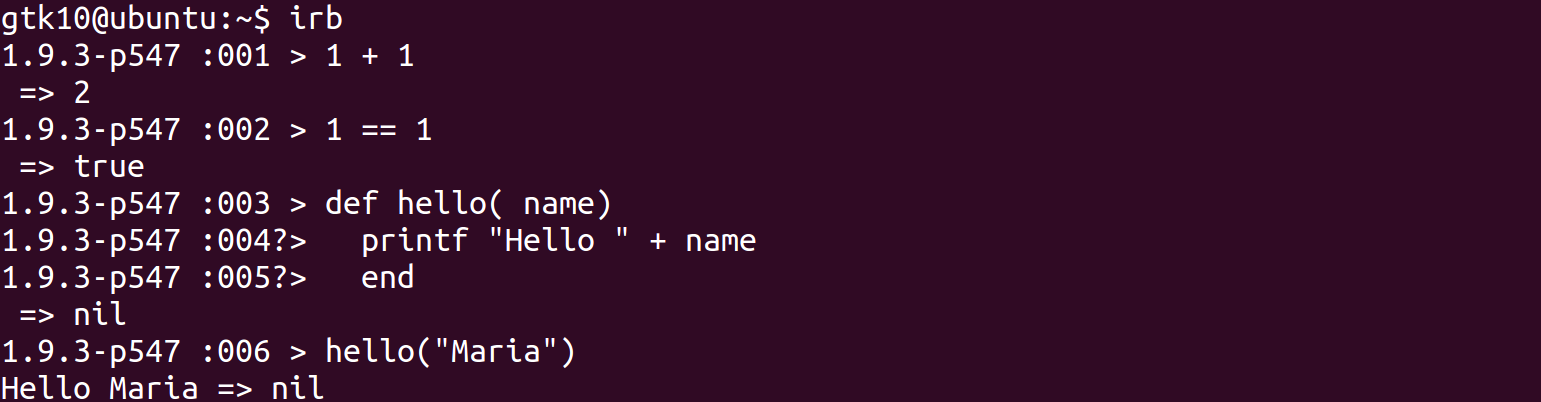
\includegraphics[scale=0.3]{images/exemplo_de_uso_do_irb}
  \caption{Exemplo de Uso do IRB}
  \label{fig:exemplo_de_uso_do_irb}
\end{figure}
\end{comment}

\lstinputlisting[ style=customBash, caption={Exemplo de uso do IRB}, label={lst:exemplo_de_uso_do_irb}]
{codigos/exemplo_de_uso_do_irb.sh}

\begin{itemize}

\begin{comment}
 \item Primeiramente é feita a chamada da ferramenta \emph{IRB} com o comando ‘‘\emph{irb}'' no terminal.
 
 \item Depois é requisitado a soma entre ‘‘\emph{1 + 1}'' resultando em ‘‘\emph{2}''.
 
 \item Em seguida é perguntado se ‘‘\emph{1 == 1}'' resultando em ‘‘\emph{true}''.

 \item E no fim é criado uma função chamada de ‘‘\emph{hello}'' com o parâmetro ‘‘\emph{name}'' e ao se 
 chamar essa função é devolvido na tela ‘‘\emph{Hello +}'' o parâmetro passado para a função. O resultado
 pode ser visto quando se requisita ‘‘\emph{hello(‘‘Maria'')}'' e se obtem como resultado 
 ‘‘\emph{Hello Maria}''.
\end{comment}
 
  \item Primeiramente na linha ‘‘1'' é feita a chamada da ferramenta \emph{IRB} com o comando ‘‘\emph{irb}'' 
  no terminal.
 
 \item Depois na linha ‘‘2'' é requisitado a soma entre ‘‘\emph{1 + 1}'' resultando em ‘‘\emph{2}'' na linha 
 ‘‘3''.
 
 \item Em seguida na linha ‘‘4'' é verificado se ‘‘\emph{1 == 1}'' resultando em ‘‘\emph{true}'' na linha 
 ‘‘5''.

 \item E no fim entre as linhas ‘‘6'' e ‘‘8'' é criado uma função chamada de ‘‘\emph{hello}'' com o 
 parâmetro ‘‘\emph{name}'' e ao se chamar essa função é devolvido na tela ‘‘\emph{Hello}'' mais o 
 parâmetro passado para a função. O resultado pode ser visto quando se requisita 
 ‘‘\emph{hello(‘‘Maria'')}'' na linha ‘‘10'', obtendo como resultado ‘‘\emph{Hello Maria}'' na linha ‘‘11''.
 
\end{itemize}

No nosso exemplo da gema ‘‘\emph{gemtranslatetoenglish}'' fizemos alguns testes simples mostrados
na código ‘‘Código \ref{lst:teste_irb_da_gema_gemtranslatetoenglish} - Teste IRB da gema 
gemtranslatetoenglish'' explicado com mais detalhes nos itens abaixo.

\begin{comment}
\begin{figure}[ht]
  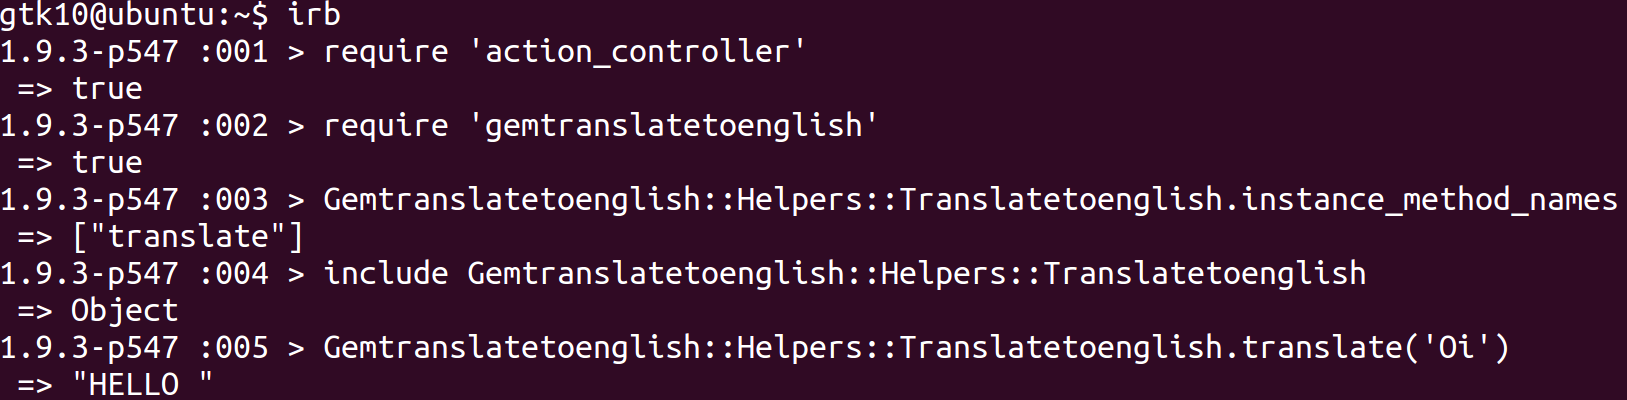
\includegraphics[scale=0.28]{images/teste_irb_da_gema_gemtranslatetoenglish.png}
  \caption{Teste IRB da gema gemtranslatetoenglish}
  \label{fig:teste_irb_da_gema_gemtranslatetoenglish}
\end{figure}
\end{comment}

\lstinputlisting[ style=customBash, caption={Teste IRB da gema gemtranslatetoenglish}, label={lst:teste_irb_da_gema_gemtranslatetoenglish}]
{codigos/teste_irb_da_gema_gemtranslatetoenglish.sh}

\begin{itemize}

 \item Primeiramente na linha ‘‘1'' é feita a chamada da ferramenta \emph{IRB} com o comando ‘‘\emph{irb}'' 
  no terminal.
  
  \item Na linha ‘‘2'' é executado o comando ‘‘ \emph{require 'action\_controller'} '' para buscar a gema 
  ‘‘\emph{ActionController}'' necessária no uso da nossa gema de exemplo quando evitamos digitar a 
  \emph{PATH} completa na ‘‘\emph{view}''.

  \item Na linha ‘‘4'' é executado o comando ‘‘ \emph{require 'gemtranslatetoenglish'} '' para buscar a 
  nossa gema de exemplo.
  
  \item Na linha ‘‘6'' é executado o comando 
  ‘‘ \emph{instance\_method\_names}'' para verificar se o nosso método \emph{translate()} existe.
  
  \item Na linha ‘‘8'' é executado o comando ‘‘\emph{include}'' para incluir as funções do módulo 
  ‘‘\emph{Translatetoenglish}''.
  
  \item Na linha ‘‘10'' é executado o comando 
  ‘‘\emph{translate('Oi')}'' para verificar se a função funciona como o esperado.
  
  \item E no fim na linha ‘‘11'' podemos verificar que a função \emph{translate()} funcionou corretamente,
  pois obtemos como resultado a palavra ‘‘\emph{HELLO }''.
  
 \end{itemize}

\subsection{Exemplo de uso de gemtranslatetoenglish}
\label{subsection:exemplo_de_uso_de_gemtranslatetoenglish}

Até o momento falamos muito da utilização do \emph{action\_controller} para simplificar o uso da função 
\emph{translate()} na \emph{view}, e agora vamos apresentar essa facilidade através de um exemplo, 
fazendo o uso da gema ‘‘\emph{gemtranslatetoenglish}'' em um projeto.

O primeiro passo é criar um projeto no \emph{framework rails} e isso pode ser feito executando 
o seguinte comando apresentado no código ‘‘Código 
\ref{lst:executa_rails_new_para_gemtranslatetoenglish} - Executa rails new para gemtranslatetoenglish''
explicado logo a seguir.

\lstinputlisting[ style=customBash, caption={Executa rails new para gemtranslatetoenglish}, label={lst:executa_rails_new_para_gemtranslatetoenglish}]
{codigos/executa_rails_new_para_gemtranslatetoenglish_simplificado.sh} 

\begin{itemize}

 \item O comando ‘‘\emph{rails new}'' implica na criação de um projeto básico do \emph{Ruby On Rails}.
 
 \item O nome ‘‘\emph{projeto\_teste\_gemtranslatetoenglish}'' é o nome do proejto a ser criado.
 
  \item Os códigos a partir da linha ‘‘2'' não representam execuções. No caso estes códigos somente 
 mostram os passos realizados por causa da execução do comando na primeira linha.
 
 \item A execução deste comando implica na criação de alguns diretórios e arquivos e por simplificação 
 somente explicaremos aqueles que vamos utilizar neste exemplo:
  
  \subitem - ‘‘\emph{Gemfile}'' arquivo que contém as \emph{gemas} que são utilizadas no projeto.
 
  \subitem - ‘‘\emph{config/routes.rb}'' arquivos que possui as rotas utilizadas no projeto.
 
\end{itemize}

Agora que criamos o projeto, precisamos fazer a criação de pelo menos um \emph{controller} e uma \emph{view}.
O \emph{controller} serve para receber uma requisição e determinar a partir dos parâmetros desta 
requisição, a \emph{view} e os dados que devem ser apresentados. A \emph{view} serve para 
determinar um formato e mostrar os dados no \emph{browser}.

Para o nosso exemplo criamos o \emph{controller} ‘‘traducao'' e a \emph{view} ‘‘index'' com a execução do 
comando que pode ser visto no código ‘‘Código \ref{lst:executa_rails_generate_para_gemtranslatetoenglish} - 
Executa rails generate para gemtranslatetoenglish'' explicado logo a seguir.

\lstinputlisting[ style=customBash, caption={Executa rails generate para gemtranslatetoenglish}, label={lst:executa_rails_generate_para_gemtranslatetoenglish}]
{codigos/executa_rails_generate_para_gemtranslatetoenglish.sh} 

\begin{itemize}

 \item Na linha ‘‘1'' é feito a execução do comando ‘‘\emph{rails generate controller traducao index}'' no 
 terminal para gerar o \emph{controller} ‘‘\emph{traducao}'', e a \emph{view} ‘‘\emph{index}'' para 
 ‘‘\emph{traducao}''.

 \item Os códigos a partir da linha ‘‘2'' não representam execuções. No caso estes códigos somente 
 mostram os passos realizados por causa da execução do comando na primeira linha.
 
 \item Na linha ‘‘2'' foi criado o \emph{controller} com o nome ‘‘\emph{traducao\_controller.rb}''
 
 \item Na linha ‘‘3'' foi adicionado no arquivo ‘‘\emph{config/routes.rb} o método \emph{get} para a 
 \emph{view} ‘‘\emph{traducao/index}''.
 
 \item Na linha ‘‘6'' foi criado a \emph{view} ‘‘\emph{traducao/index.html.erb}''.
 
 \item A partir da linha ‘‘7'' são criados os arquivos de teste funcional, os \emph{helpers}, e os 
 \emph{assets} que possuem códigos \emph{coffeescript} que depois vão se tornar \emph{javascript} e 
 \emph{scss} que depois vão se tornar \emph{css}.
 
\end{itemize}


Agora para fazer o uso da nossa gema de exemplo em um projeto feito no \emph{Ruby On Rails}, basta fazer a 
inclusão da gema no final do arquivo \emph{Gemfile} da mesma forma como mostrado no código ‘‘Código 
\ref{lst:adiciona_gemtranslatetoenglish_no_gemfile} - Adiciona gemtranslatetoenglish no Gemfile''
 
 \lstinputlisting[ style=customRuby, caption={Adiciona gemtranslatetoenglish no Gemfile}, label={lst:adiciona_gemtranslatetoenglish_no_gemfile}]
{codigos/adiciona_gemtranslatetoenglish_no_gemfile}
 
Agora que a gema ‘‘\emph{gemtranslatetoenglish}'' já esta incluída no nosso projeto, podemos fazer o uso 
dela em uma \emph{view} da seguinte maneira apresentada no código ‘‘Código 
\ref{lst:exemplo_do_translate_na_view} - Exemplo do translate() na view'' explicado logo a seguir.

\lstinputlisting[ style=customRubyHTML, caption={Exemplo do translate() na view}, label={lst:exemplo_do_translate_na_view}]
{codigos/projeto_teste_gemtranslatetoenglish/app/views/traducao/index.html.erb} 
 
 \begin{itemize}
 
  \item As linhas ‘‘1'' e ‘‘2'' já existiam, pois foram criadas automaticamente após a execução do comando 
  ‘‘\emph{rails generate controller traducao index}'' que mostramos no código ‘‘Código 
  \ref{lst:executa_rails_generate_para_gemtranslatetoenglish} - Executa rails generate para 
  gemtranslatetoenglish''.
  
  \item Na linha ‘‘4'' inserimos uma \emph{tag <p>} indicando para o \emph{browser} que vamos inserir um 
  texto. Depois inserimos a \emph{tag <\%= ... \%>} que indica que entre essas \emph{tags} será inserido um 
  código \emph{Ruby}. E dentro destas \emph{tags} chamamos o nosso método \emph{translate()} da gema 
  ‘‘\emph{gemtranslatetoenglish}'' com o parâmetro ‘‘Oi Mundo''.
  
 \end{itemize}

Agora que temos a nossa função ‘‘\emph{translate()}'' dentro da \emph{view} ‘‘\emph{traducao/index}'', podemos 
verificar se a tradução funciona corretamente. Para isso devemos dentro do diretório do nosso projeto,
iniciar o servidor no terminal através do comando ‘‘\emph{rails server -p2342}'', onde o parâmetro ‘‘-p2342'' 
indica que o servidor vai usar a porta ‘‘2342''. 

Depois com o servidor funcionando, podemos verificar na imagem ‘‘Figure \ref{fig:resultado_de_translate_na_view} - 
Resultado de Translate na View'' que ao se acessar o endereço ‘‘localhost:2342/traducao/index'' no 
\emph{browser}, a nossa função de tradução funciona corretamente, pois na página é apresentado o 
texto ‘‘HELLO WORLD''.
 
 \begin{figure}[ht]
  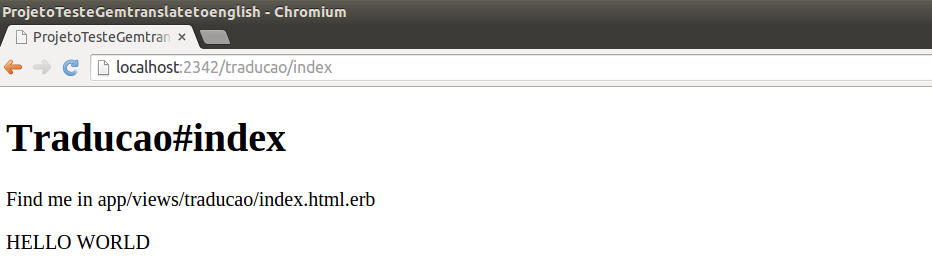
\includegraphics[scale=0.49]{images/resultado_de_translate_na_view.png}
  \caption{Resultado de Translate na View}
  \label{fig:resultado_de_translate_na_view}
\end{figure}